\documentclass[twoside]{book}

% Packages required by doxygen
\usepackage{fixltx2e}
\usepackage{calc}
\usepackage{doxygen}
\usepackage[export]{adjustbox} % also loads graphicx
\usepackage{graphicx}
\usepackage[utf8]{inputenc}
\usepackage{makeidx}
\usepackage{multicol}
\usepackage{multirow}
\PassOptionsToPackage{warn}{textcomp}
\usepackage{textcomp}
\usepackage[nointegrals]{wasysym}
\usepackage[table]{xcolor}

% Font selection
\usepackage[T1]{fontenc}
\usepackage[scaled=.90]{helvet}
\usepackage{courier}
\usepackage{amssymb}
\usepackage{sectsty}
\renewcommand{\familydefault}{\sfdefault}
\allsectionsfont{%
  \fontseries{bc}\selectfont%
  \color{darkgray}%
}
\renewcommand{\DoxyLabelFont}{%
  \fontseries{bc}\selectfont%
  \color{darkgray}%
}
\newcommand{\+}{\discretionary{\mbox{\scriptsize$\hookleftarrow$}}{}{}}

% Page & text layout
\usepackage{geometry}
\geometry{%
  a4paper,%
  top=2.5cm,%
  bottom=2.5cm,%
  left=2.5cm,%
  right=2.5cm%
}
\tolerance=750
\hfuzz=15pt
\hbadness=750
\setlength{\emergencystretch}{15pt}
\setlength{\parindent}{0cm}
\setlength{\parskip}{3ex plus 2ex minus 2ex}
\makeatletter
\renewcommand{\paragraph}{%
  \@startsection{paragraph}{4}{0ex}{-1.0ex}{1.0ex}{%
    \normalfont\normalsize\bfseries\SS@parafont%
  }%
}
\renewcommand{\subparagraph}{%
  \@startsection{subparagraph}{5}{0ex}{-1.0ex}{1.0ex}{%
    \normalfont\normalsize\bfseries\SS@subparafont%
  }%
}
\makeatother

% Headers & footers
\usepackage{fancyhdr}
\pagestyle{fancyplain}
\fancyhead[LE]{\fancyplain{}{\bfseries\thepage}}
\fancyhead[CE]{\fancyplain{}{}}
\fancyhead[RE]{\fancyplain{}{\bfseries\leftmark}}
\fancyhead[LO]{\fancyplain{}{\bfseries\rightmark}}
\fancyhead[CO]{\fancyplain{}{}}
\fancyhead[RO]{\fancyplain{}{\bfseries\thepage}}
\fancyfoot[LE]{\fancyplain{}{}}
\fancyfoot[CE]{\fancyplain{}{}}
\fancyfoot[RE]{\fancyplain{}{\bfseries\scriptsize Generated by Doxygen }}
\fancyfoot[LO]{\fancyplain{}{\bfseries\scriptsize Generated by Doxygen }}
\fancyfoot[CO]{\fancyplain{}{}}
\fancyfoot[RO]{\fancyplain{}{}}
\renewcommand{\footrulewidth}{0.4pt}
\renewcommand{\chaptermark}[1]{%
  \markboth{#1}{}%
}
\renewcommand{\sectionmark}[1]{%
  \markright{\thesection\ #1}%
}

% Indices & bibliography
\usepackage{natbib}
\usepackage[titles]{tocloft}
\setcounter{tocdepth}{3}
\setcounter{secnumdepth}{5}
\makeindex

% Hyperlinks (required, but should be loaded last)
\usepackage{ifpdf}
\ifpdf
  \usepackage[pdftex,pagebackref=true]{hyperref}
\else
  \usepackage[ps2pdf,pagebackref=true]{hyperref}
\fi
\hypersetup{%
  colorlinks=true,%
  linkcolor=blue,%
  citecolor=blue,%
  unicode%
}

% Custom commands
\newcommand{\clearemptydoublepage}{%
  \newpage{\pagestyle{empty}\cleardoublepage}%
}

\usepackage{caption}
\captionsetup{labelsep=space,justification=centering,font={bf},singlelinecheck=off,skip=4pt,position=top}

%===== C O N T E N T S =====

\begin{document}

% Titlepage & ToC
\hypersetup{pageanchor=false,
             bookmarksnumbered=true,
             pdfencoding=unicode
            }
\pagenumbering{roman}
\begin{titlepage}
\vspace*{7cm}
\begin{center}%
{\Large Árbol B+ }\\
\vspace*{1cm}
{\large Generated by Doxygen 1.8.11}\\
\end{center}
\end{titlepage}
\clearemptydoublepage
\tableofcontents
\clearemptydoublepage
\pagenumbering{arabic}
\hypersetup{pageanchor=true}

%--- Begin generated contents ---
\chapter{Hierarchical Index}
\section{Class Hierarchy}
This inheritance list is sorted roughly, but not completely, alphabetically\+:\begin{DoxyCompactList}
\item \contentsline{section}{Animal}{\pageref{classAnimal}}{}
\begin{DoxyCompactList}
\item \contentsline{section}{Lobo}{\pageref{classLobo}}{}
\item \contentsline{section}{Oveja}{\pageref{classOveja}}{}
\item \contentsline{section}{Raton}{\pageref{classRaton}}{}
\item \contentsline{section}{Zorro}{\pageref{classZorro}}{}
\end{DoxyCompactList}
\item \contentsline{section}{Celda}{\pageref{classCelda}}{}
\item \contentsline{section}{Controlador}{\pageref{classControlador}}{}
\end{DoxyCompactList}

\chapter{Data Structure Index}
\section{Data Structures}
Here are the data structures with brief descriptions\+:\begin{DoxyCompactList}
\item\contentsline{section}{\hyperlink{classBPlusTree}{B\+Plus\+Tree$<$ Data $>$} }{\pageref{classBPlusTree}}{}
\item\contentsline{section}{\hyperlink{classLeaf}{Leaf$<$ Data $>$} }{\pageref{classLeaf}}{}
\item\contentsline{section}{\hyperlink{classNode}{Node$<$ Data $>$} }{\pageref{classNode}}{}
\end{DoxyCompactList}

\chapter{File Index}
\section{File List}
Here is a list of all files with brief descriptions\+:\begin{DoxyCompactList}
\item\contentsline{section}{\hyperlink{BPlusTree_8h}{B\+Plus\+Tree.\+h} }{\pageref{BPlusTree_8h}}{}
\item\contentsline{section}{\hyperlink{Leaf_8h}{Leaf.\+h} }{\pageref{Leaf_8h}}{}
\item\contentsline{section}{\hyperlink{main_8cpp}{main.\+cpp} }{\pageref{main_8cpp}}{}
\item\contentsline{section}{\hyperlink{Node_8h}{Node.\+h} \\*Clase Arbol\+B+ }{\pageref{Node_8h}}{}
\end{DoxyCompactList}

\chapter{Data Structure Documentation}
\hypertarget{classBPlusTree}{}\section{B\+Plus\+Tree$<$ Data $>$ Class Template Reference}
\label{classBPlusTree}\index{B\+Plus\+Tree$<$ Data $>$@{B\+Plus\+Tree$<$ Data $>$}}


{\ttfamily \#include $<$B\+Plus\+Tree.\+h$>$}

\subsection*{Public Member Functions}
\begin{DoxyCompactItemize}
\item 
\hyperlink{classBPlusTree_a6a178fd510a5f67356e94ae9ae75ab5b}{B\+Plus\+Tree} ()
\begin{DoxyCompactList}\small\item\em Constructor por defecto. \end{DoxyCompactList}\item 
\hyperlink{classBPlusTree_a8e72d749013aed34df0e4a166ec431f5}{B\+Plus\+Tree} (int \hyperlink{classBPlusTree_a5c36dd5810d348dc87c106323311b1c5}{order})
\begin{DoxyCompactList}\small\item\em Constructor para crear un Arbol de un orden pre establecido. \end{DoxyCompactList}\item 
virtual \hyperlink{classBPlusTree_a33800c9324716875143eff1655b7ded0}{$\sim$\+B\+Plus\+Tree} ()
\begin{DoxyCompactList}\small\item\em Destructor. \end{DoxyCompactList}\item 
void \hyperlink{classBPlusTree_a4a5da00290010f91715426f17953fa73}{aux\+Destructor} (\hyperlink{classNode}{Node}$<$ \hyperlink{main_8cpp_a0c209e815d35b218025a240523b4335b}{Data} $>$ $\ast$node)
\begin{DoxyCompactList}\small\item\em Metodo auxiliar del destructor de la clase. \end{DoxyCompactList}\item 
void \hyperlink{classBPlusTree_ab980a458ae890fcebe8557a887fc14f4}{insert\+Ak7} (int key)
\begin{DoxyCompactList}\small\item\em Metodo para insertar un dato al arbol. \end{DoxyCompactList}\item 
void \hyperlink{classBPlusTree_ad2fc2c2dfe80e853f51827095d88808a}{aux\+Insert\+Ak7} (int key, \hyperlink{classNode}{Node}$<$ \hyperlink{main_8cpp_a0c209e815d35b218025a240523b4335b}{Data} $>$ $\ast$node)
\begin{DoxyCompactList}\small\item\em Metodo para insertar un dato al arbol. \end{DoxyCompactList}\item 
void \hyperlink{classBPlusTree_afa91ee0ef70f54bcfe087a9c894edcd2}{split\+Ak7} (\hyperlink{classNode}{Node}$<$ \hyperlink{main_8cpp_a0c209e815d35b218025a240523b4335b}{Data} $>$ $\ast$node, int key, \hyperlink{classNode}{Node}$<$ \hyperlink{main_8cpp_a0c209e815d35b218025a240523b4335b}{Data} $>$ $\ast$old\+Son, \hyperlink{classNode}{Node}$<$ \hyperlink{main_8cpp_a0c209e815d35b218025a240523b4335b}{Data} $>$ $\ast$new\+Son)
\begin{DoxyCompactList}\small\item\em Metodo que divide un nodo al ingresar una llave. \end{DoxyCompactList}\item 
int \hyperlink{classBPlusTree_a78301c77d2aee16039680ba1e65718af}{pointer\+To\+Go} (int key, \hyperlink{classNode}{Node}$<$ \hyperlink{main_8cpp_a0c209e815d35b218025a240523b4335b}{Data} $>$ $\ast$node)
\begin{DoxyCompactList}\small\item\em Metodo que dice a cual nodo del arreglo de punteros de nodos hay que ir al meter una llave. \end{DoxyCompactList}\item 
int $\ast$ \hyperlink{classBPlusTree_a390038248adfe3d85ab2c25015ce07e3}{array\+To\+Split\+Func} (\hyperlink{classNode}{Node}$<$ \hyperlink{main_8cpp_a0c209e815d35b218025a240523b4335b}{Data} $>$ $\ast$node, int key)
\begin{DoxyCompactList}\small\item\em Metodo que crea el arreglo que luego hay que dividir. \end{DoxyCompactList}\item 
void \hyperlink{classBPlusTree_aca5abac752f2e91b8d9642d145dc8c74}{delete\+First\+Element} (int $\ast$array, int size)
\begin{DoxyCompactList}\small\item\em Metodo que elimina el primer dato de un arreglo. \end{DoxyCompactList}\item 
int \hyperlink{classBPlusTree_af72ca8a996a12aaf3875717b35ddba4d}{amount\+Elements} (int $\ast$array, int size)
\begin{DoxyCompactList}\small\item\em Metodo que devuelve la cantidad de elementos de un arreglo. \end{DoxyCompactList}\item 
void \hyperlink{classBPlusTree_a300ff0b8ea4244bc2f67a0706f0c934e}{assign\+Downward\+Ptrs} (\hyperlink{classNode}{Node}$<$ \hyperlink{main_8cpp_a0c209e815d35b218025a240523b4335b}{Data} $>$ $\ast$old, \hyperlink{classNode}{Node}$<$ \hyperlink{main_8cpp_a0c209e815d35b218025a240523b4335b}{Data} $>$ $\ast$new\+One, \hyperlink{classNode}{Node}$<$ \hyperlink{main_8cpp_a0c209e815d35b218025a240523b4335b}{Data} $>$ $\ast$old\+Son, \hyperlink{classNode}{Node}$<$ \hyperlink{main_8cpp_a0c209e815d35b218025a240523b4335b}{Data} $>$ $\ast$new\+Son, int key)
\begin{DoxyCompactList}\small\item\em Metodo que arregla los punteros hacia abajo de un nodo dividido. \end{DoxyCompactList}\item 
int \hyperlink{classBPlusTree_ac31a935a665736906ad9725b2b603f7d}{position\+Of\+Key} (int key, \hyperlink{classNode}{Node}$<$ \hyperlink{main_8cpp_a0c209e815d35b218025a240523b4335b}{Data} $>$ $\ast$node)
\begin{DoxyCompactList}\small\item\em Metodo que dice en que posicion qeudo la llave. \end{DoxyCompactList}\item 
void \hyperlink{classBPlusTree_a806305a534da3c3809849b09bf8e7feb}{father\+Ptrs} (\hyperlink{classNode}{Node}$<$ \hyperlink{main_8cpp_a0c209e815d35b218025a240523b4335b}{Data} $>$ $\ast$node)
\begin{DoxyCompactList}\small\item\em Metodo que asigna el correspondiente padre de un nodo. \end{DoxyCompactList}\item 
void \hyperlink{classBPlusTree_ad90c387310153b5199e297d38a6c9901}{sort} (int $\ast$array, int size)
\begin{DoxyCompactList}\small\item\em Metodo que ordena un arreglo con un selection sort. \end{DoxyCompactList}\item 
void \hyperlink{classBPlusTree_a73ac50b1543b2240198524fb3221f78c}{special\+Sort} (int $\ast$array, \hyperlink{classNode}{Node}$<$ \hyperlink{main_8cpp_a0c209e815d35b218025a240523b4335b}{Data} $>$ $\ast$$\ast$array\+Ptrs, \hyperlink{classNode}{Node}$<$ \hyperlink{main_8cpp_a0c209e815d35b218025a240523b4335b}{Data} $>$ $\ast$left, \hyperlink{classNode}{Node}$<$ \hyperlink{main_8cpp_a0c209e815d35b218025a240523b4335b}{Data} $>$ $\ast$right, int size)
\begin{DoxyCompactList}\small\item\em Metodo que ordena un arreglo con un selection sort y arregla los punteros de los elementos que se mueven. \end{DoxyCompactList}\item 
void \hyperlink{classBPlusTree_a03b52c1a8321da333a0fd3af5b486cc2}{delete\+Ak7} (int key)
\begin{DoxyCompactList}\small\item\em Metodo que elimina un dato del arbol. \end{DoxyCompactList}\item 
void \hyperlink{classBPlusTree_a0f96068cb3a0aa30fc0fd137d29dd092}{aux\+Delete} (int key, \hyperlink{classNode}{Node}$<$ \hyperlink{main_8cpp_a0c209e815d35b218025a240523b4335b}{Data} $>$ $\ast$node)
\begin{DoxyCompactList}\small\item\em Metodo auxiliar que elimina un dato del arbol. \end{DoxyCompactList}\item 
void \hyperlink{classBPlusTree_a595d1cc4c48e93347297fbc252fa4fd8}{merge} (int key)
\begin{DoxyCompactList}\small\item\em Metodo para unir dos nodos u hojas. \end{DoxyCompactList}\item 
void \hyperlink{classBPlusTree_aa0fb08b95e3a6186328f71e58c76c274}{key\+From\+Sibling} (int key, \hyperlink{classNode}{Node}$<$ \hyperlink{main_8cpp_a0c209e815d35b218025a240523b4335b}{Data} $>$ $\ast$node, \hyperlink{classNode}{Node}$<$ \hyperlink{main_8cpp_a0c209e815d35b218025a240523b4335b}{Data} $>$ $\ast$Sibling)
\begin{DoxyCompactList}\small\item\em Metodo que busca el elemento del hermano a obtener y lo coloca en el nodo en cuestion. \end{DoxyCompactList}\item 
\hyperlink{classNode}{Node}$<$ \hyperlink{main_8cpp_a0c209e815d35b218025a240523b4335b}{Data} $>$ $\ast$ \hyperlink{classBPlusTree_a16141dce1872e3284360ee9dadccbf66}{find\+My\+Sibling} (\hyperlink{classNode}{Node}$<$ \hyperlink{main_8cpp_a0c209e815d35b218025a240523b4335b}{Data} $>$ $\ast$node, int key)
\begin{DoxyCompactList}\small\item\em Metodo que devuelve el nodo hermano. \end{DoxyCompactList}\item 
void \hyperlink{classBPlusTree_a4011c6ed03d299990a5f6dcad94451ef}{delete\+From\+Father} (\hyperlink{classNode}{Node}$<$ \hyperlink{main_8cpp_a0c209e815d35b218025a240523b4335b}{Data} $>$ $\ast$node, int key, int new\+Key)
\begin{DoxyCompactList}\small\item\em Metodo que borra la llave del padre. \end{DoxyCompactList}\item 
void \hyperlink{classBPlusTree_a27560590ee9fcc9497e793dae64b44e6}{sort\+With\+Minus\+One} (int $\ast$array, int size)
\begin{DoxyCompactList}\small\item\em Metodo para ordenar un arreglo con un menos uno entre las llaves. \end{DoxyCompactList}\item 
void \hyperlink{classBPlusTree_ae462ff062f5bd67ddd8d100f7c1a761e}{print\+Tree} ()
\begin{DoxyCompactList}\small\item\em Metodo para imprimir el arbol. \end{DoxyCompactList}\item 
void \hyperlink{classBPlusTree_a89ab7badee19297ca31dfd571a0467e3}{aux\+Print} (\hyperlink{classNode}{Node}$<$ \hyperlink{main_8cpp_a0c209e815d35b218025a240523b4335b}{Data} $>$ $\ast$node, int level, int index)
\begin{DoxyCompactList}\small\item\em Metodo auxiliar para imprimir el arbol. \end{DoxyCompactList}\item 
bool \hyperlink{classBPlusTree_a34b5caf4d18027d5bb0cf7ad43203281}{find} (int key)
\begin{DoxyCompactList}\small\item\em Metodo para buscar un dato. \end{DoxyCompactList}\item 
bool \hyperlink{classBPlusTree_a0fdb6565dc2283aebe4097ba46735f36}{aux\+Find} (int key, \hyperlink{classNode}{Node}$<$ \hyperlink{main_8cpp_a0c209e815d35b218025a240523b4335b}{Data} $>$ $\ast$node)
\begin{DoxyCompactList}\small\item\em Metodo auxiliar para buscar un dato. \end{DoxyCompactList}\end{DoxyCompactItemize}
\subsection*{Data Fields}
\begin{DoxyCompactItemize}
\item 
\hyperlink{classNode}{Node}$<$ \hyperlink{main_8cpp_a0c209e815d35b218025a240523b4335b}{Data} $>$ $\ast$ \hyperlink{classBPlusTree_a902548acb47c9268aec2419341ea472a}{root}
\item 
int \hyperlink{classBPlusTree_a54b32b4ed373559b4e0821ffced9de86}{levels}
\item 
int \hyperlink{classBPlusTree_a5c36dd5810d348dc87c106323311b1c5}{order}
\item 
int \hyperlink{classBPlusTree_af012b8daf299c534b1b439d20b5343f6}{tree\+Elements}
\end{DoxyCompactItemize}


\subsection{Constructor \& Destructor Documentation}
\index{B\+Plus\+Tree@{B\+Plus\+Tree}!B\+Plus\+Tree@{B\+Plus\+Tree}}
\index{B\+Plus\+Tree@{B\+Plus\+Tree}!B\+Plus\+Tree@{B\+Plus\+Tree}}
\subsubsection[{\texorpdfstring{B\+Plus\+Tree()}{BPlusTree()}}]{\setlength{\rightskip}{0pt plus 5cm}template$<$typename Data $>$ {\bf B\+Plus\+Tree}$<$ {\bf Data} $>$\+::{\bf B\+Plus\+Tree} (
\begin{DoxyParamCaption}
{}
\end{DoxyParamCaption}
)\hspace{0.3cm}{\ttfamily [inline]}}\hypertarget{classBPlusTree_a6a178fd510a5f67356e94ae9ae75ab5b}{}\label{classBPlusTree_a6a178fd510a5f67356e94ae9ae75ab5b}


Constructor por defecto. 

\index{B\+Plus\+Tree@{B\+Plus\+Tree}!B\+Plus\+Tree@{B\+Plus\+Tree}}
\index{B\+Plus\+Tree@{B\+Plus\+Tree}!B\+Plus\+Tree@{B\+Plus\+Tree}}
\subsubsection[{\texorpdfstring{B\+Plus\+Tree(int order)}{BPlusTree(int order)}}]{\setlength{\rightskip}{0pt plus 5cm}template$<$typename Data $>$ {\bf B\+Plus\+Tree}$<$ {\bf Data} $>$\+::{\bf B\+Plus\+Tree} (
\begin{DoxyParamCaption}
\item[{int}]{order}
\end{DoxyParamCaption}
)\hspace{0.3cm}{\ttfamily [inline]}}\hypertarget{classBPlusTree_a8e72d749013aed34df0e4a166ec431f5}{}\label{classBPlusTree_a8e72d749013aed34df0e4a166ec431f5}


Constructor para crear un Arbol de un orden pre establecido. 

\index{B\+Plus\+Tree@{B\+Plus\+Tree}!````~B\+Plus\+Tree@{$\sim$\+B\+Plus\+Tree}}
\index{````~B\+Plus\+Tree@{$\sim$\+B\+Plus\+Tree}!B\+Plus\+Tree@{B\+Plus\+Tree}}
\subsubsection[{\texorpdfstring{$\sim$\+B\+Plus\+Tree()}{~BPlusTree()}}]{\setlength{\rightskip}{0pt plus 5cm}template$<$typename Data $>$ virtual {\bf B\+Plus\+Tree}$<$ {\bf Data} $>$\+::$\sim${\bf B\+Plus\+Tree} (
\begin{DoxyParamCaption}
{}
\end{DoxyParamCaption}
)\hspace{0.3cm}{\ttfamily [inline]}, {\ttfamily [virtual]}}\hypertarget{classBPlusTree_a33800c9324716875143eff1655b7ded0}{}\label{classBPlusTree_a33800c9324716875143eff1655b7ded0}


Destructor. 



\subsection{Member Function Documentation}
\index{B\+Plus\+Tree@{B\+Plus\+Tree}!amount\+Elements@{amount\+Elements}}
\index{amount\+Elements@{amount\+Elements}!B\+Plus\+Tree@{B\+Plus\+Tree}}
\subsubsection[{\texorpdfstring{amount\+Elements(int $\ast$array, int size)}{amountElements(int *array, int size)}}]{\setlength{\rightskip}{0pt plus 5cm}template$<$typename Data $>$ int {\bf B\+Plus\+Tree}$<$ {\bf Data} $>$\+::amount\+Elements (
\begin{DoxyParamCaption}
\item[{int $\ast$}]{array, }
\item[{int}]{size}
\end{DoxyParamCaption}
)\hspace{0.3cm}{\ttfamily [inline]}}\hypertarget{classBPlusTree_af72ca8a996a12aaf3875717b35ddba4d}{}\label{classBPlusTree_af72ca8a996a12aaf3875717b35ddba4d}


Metodo que devuelve la cantidad de elementos de un arreglo. 


\begin{DoxyParams}{Parameters}
{\em array} & Arreglo al que hay que contarle la cantidad de elementos. \\
\hline
{\em size} & Tamanno del arreglo. \\
\hline
\end{DoxyParams}
\begin{DoxyReturn}{Returns}
Cantidad de elementos del arreglo. 
\end{DoxyReturn}
\index{B\+Plus\+Tree@{B\+Plus\+Tree}!array\+To\+Split\+Func@{array\+To\+Split\+Func}}
\index{array\+To\+Split\+Func@{array\+To\+Split\+Func}!B\+Plus\+Tree@{B\+Plus\+Tree}}
\subsubsection[{\texorpdfstring{array\+To\+Split\+Func(\+Node$<$ Data $>$ $\ast$node, int key)}{arrayToSplitFunc(Node< Data > *node, int key)}}]{\setlength{\rightskip}{0pt plus 5cm}template$<$typename Data $>$ int$\ast$ {\bf B\+Plus\+Tree}$<$ {\bf Data} $>$\+::array\+To\+Split\+Func (
\begin{DoxyParamCaption}
\item[{{\bf Node}$<$ {\bf Data} $>$ $\ast$}]{node, }
\item[{int}]{key}
\end{DoxyParamCaption}
)\hspace{0.3cm}{\ttfamily [inline]}}\hypertarget{classBPlusTree_a390038248adfe3d85ab2c25015ce07e3}{}\label{classBPlusTree_a390038248adfe3d85ab2c25015ce07e3}


Metodo que crea el arreglo que luego hay que dividir. 


\begin{DoxyParams}{Parameters}
{\em node} & Nodo que esta lleno. \\
\hline
{\em key} & Llave que tiene que agregar a las llaves del node. \\
\hline
\end{DoxyParams}
\begin{DoxyReturn}{Returns}
Arreglo de enteros que hay que dividir. 
\end{DoxyReturn}
\index{B\+Plus\+Tree@{B\+Plus\+Tree}!assign\+Downward\+Ptrs@{assign\+Downward\+Ptrs}}
\index{assign\+Downward\+Ptrs@{assign\+Downward\+Ptrs}!B\+Plus\+Tree@{B\+Plus\+Tree}}
\subsubsection[{\texorpdfstring{assign\+Downward\+Ptrs(\+Node$<$ Data $>$ $\ast$old, Node$<$ Data $>$ $\ast$new\+One, Node$<$ Data $>$ $\ast$old\+Son, Node$<$ Data $>$ $\ast$new\+Son, int key)}{assignDownwardPtrs(Node< Data > *old, Node< Data > *newOne, Node< Data > *oldSon, Node< Data > *newSon, int key)}}]{\setlength{\rightskip}{0pt plus 5cm}template$<$typename Data $>$ void {\bf B\+Plus\+Tree}$<$ {\bf Data} $>$\+::assign\+Downward\+Ptrs (
\begin{DoxyParamCaption}
\item[{{\bf Node}$<$ {\bf Data} $>$ $\ast$}]{old, }
\item[{{\bf Node}$<$ {\bf Data} $>$ $\ast$}]{new\+One, }
\item[{{\bf Node}$<$ {\bf Data} $>$ $\ast$}]{old\+Son, }
\item[{{\bf Node}$<$ {\bf Data} $>$ $\ast$}]{new\+Son, }
\item[{int}]{key}
\end{DoxyParamCaption}
)\hspace{0.3cm}{\ttfamily [inline]}}\hypertarget{classBPlusTree_a300ff0b8ea4244bc2f67a0706f0c934e}{}\label{classBPlusTree_a300ff0b8ea4244bc2f67a0706f0c934e}


Metodo que arregla los punteros hacia abajo de un nodo dividido. 


\begin{DoxyParams}{Parameters}
{\em old} & Nodo ya existente del nodo dividido. \\
\hline
{\em new\+One} & Nodo nuevo creado al dividir el nodo viejo. \\
\hline
{\em old\+Son} & El hijo del nodo viejo que ya existia al dividirse el nodo hijo viejo. \\
\hline
{\em new\+Son} & El hijo del nodo viejo que habia sido creado al dividirse el nodo hijo viejo \\
\hline
{\em key} & la llave. \\
\hline
\end{DoxyParams}
\index{B\+Plus\+Tree@{B\+Plus\+Tree}!aux\+Delete@{aux\+Delete}}
\index{aux\+Delete@{aux\+Delete}!B\+Plus\+Tree@{B\+Plus\+Tree}}
\subsubsection[{\texorpdfstring{aux\+Delete(int key, Node$<$ Data $>$ $\ast$node)}{auxDelete(int key, Node< Data > *node)}}]{\setlength{\rightskip}{0pt plus 5cm}template$<$typename Data $>$ void {\bf B\+Plus\+Tree}$<$ {\bf Data} $>$\+::aux\+Delete (
\begin{DoxyParamCaption}
\item[{int}]{key, }
\item[{{\bf Node}$<$ {\bf Data} $>$ $\ast$}]{node}
\end{DoxyParamCaption}
)\hspace{0.3cm}{\ttfamily [inline]}}\hypertarget{classBPlusTree_a0f96068cb3a0aa30fc0fd137d29dd092}{}\label{classBPlusTree_a0f96068cb3a0aa30fc0fd137d29dd092}


Metodo auxiliar que elimina un dato del arbol. 


\begin{DoxyParams}{Parameters}
{\em key} & Llave que se va a eliminar. \\
\hline
{\em node} & Nodo en el que se verifica si la llave esta para eliminar. \\
\hline
\end{DoxyParams}
\index{B\+Plus\+Tree@{B\+Plus\+Tree}!aux\+Destructor@{aux\+Destructor}}
\index{aux\+Destructor@{aux\+Destructor}!B\+Plus\+Tree@{B\+Plus\+Tree}}
\subsubsection[{\texorpdfstring{aux\+Destructor(\+Node$<$ Data $>$ $\ast$node)}{auxDestructor(Node< Data > *node)}}]{\setlength{\rightskip}{0pt plus 5cm}template$<$typename Data $>$ void {\bf B\+Plus\+Tree}$<$ {\bf Data} $>$\+::aux\+Destructor (
\begin{DoxyParamCaption}
\item[{{\bf Node}$<$ {\bf Data} $>$ $\ast$}]{node}
\end{DoxyParamCaption}
)\hspace{0.3cm}{\ttfamily [inline]}}\hypertarget{classBPlusTree_a4a5da00290010f91715426f17953fa73}{}\label{classBPlusTree_a4a5da00290010f91715426f17953fa73}


Metodo auxiliar del destructor de la clase. 


\begin{DoxyParams}{Parameters}
{\em node} & Nodo al cual le debe elmiminar los nodos que apunta y a si misma. \\
\hline
\end{DoxyParams}
\index{B\+Plus\+Tree@{B\+Plus\+Tree}!aux\+Find@{aux\+Find}}
\index{aux\+Find@{aux\+Find}!B\+Plus\+Tree@{B\+Plus\+Tree}}
\subsubsection[{\texorpdfstring{aux\+Find(int key, Node$<$ Data $>$ $\ast$node)}{auxFind(int key, Node< Data > *node)}}]{\setlength{\rightskip}{0pt plus 5cm}template$<$typename Data $>$ bool {\bf B\+Plus\+Tree}$<$ {\bf Data} $>$\+::aux\+Find (
\begin{DoxyParamCaption}
\item[{int}]{key, }
\item[{{\bf Node}$<$ {\bf Data} $>$ $\ast$}]{node}
\end{DoxyParamCaption}
)\hspace{0.3cm}{\ttfamily [inline]}}\hypertarget{classBPlusTree_a0fdb6565dc2283aebe4097ba46735f36}{}\label{classBPlusTree_a0fdb6565dc2283aebe4097ba46735f36}


Metodo auxiliar para buscar un dato. 


\begin{DoxyParams}{Parameters}
{\em key} & Llave que se busca. \\
\hline
{\em node} & Nodo en donde se busca la llave. \\
\hline
\end{DoxyParams}
\begin{DoxyReturn}{Returns}
Si se encontro el dato. 
\end{DoxyReturn}
\index{B\+Plus\+Tree@{B\+Plus\+Tree}!aux\+Insert\+Ak7@{aux\+Insert\+Ak7}}
\index{aux\+Insert\+Ak7@{aux\+Insert\+Ak7}!B\+Plus\+Tree@{B\+Plus\+Tree}}
\subsubsection[{\texorpdfstring{aux\+Insert\+Ak7(int key, Node$<$ Data $>$ $\ast$node)}{auxInsertAk7(int key, Node< Data > *node)}}]{\setlength{\rightskip}{0pt plus 5cm}template$<$typename Data $>$ void {\bf B\+Plus\+Tree}$<$ {\bf Data} $>$\+::aux\+Insert\+Ak7 (
\begin{DoxyParamCaption}
\item[{int}]{key, }
\item[{{\bf Node}$<$ {\bf Data} $>$ $\ast$}]{node}
\end{DoxyParamCaption}
)\hspace{0.3cm}{\ttfamily [inline]}}\hypertarget{classBPlusTree_ad2fc2c2dfe80e853f51827095d88808a}{}\label{classBPlusTree_ad2fc2c2dfe80e853f51827095d88808a}


Metodo para insertar un dato al arbol. 


\begin{DoxyParams}{Parameters}
{\em key} & Llave que se va a insertar al arbol. \\
\hline
{\em node} & Nodo en el cual se va a tratar de insertar la llave. \\
\hline
\end{DoxyParams}
\index{B\+Plus\+Tree@{B\+Plus\+Tree}!aux\+Print@{aux\+Print}}
\index{aux\+Print@{aux\+Print}!B\+Plus\+Tree@{B\+Plus\+Tree}}
\subsubsection[{\texorpdfstring{aux\+Print(\+Node$<$ Data $>$ $\ast$node, int level, int index)}{auxPrint(Node< Data > *node, int level, int index)}}]{\setlength{\rightskip}{0pt plus 5cm}template$<$typename Data $>$ void {\bf B\+Plus\+Tree}$<$ {\bf Data} $>$\+::aux\+Print (
\begin{DoxyParamCaption}
\item[{{\bf Node}$<$ {\bf Data} $>$ $\ast$}]{node, }
\item[{int}]{level, }
\item[{int}]{index}
\end{DoxyParamCaption}
)\hspace{0.3cm}{\ttfamily [inline]}}\hypertarget{classBPlusTree_a89ab7badee19297ca31dfd571a0467e3}{}\label{classBPlusTree_a89ab7badee19297ca31dfd571a0467e3}


Metodo auxiliar para imprimir el arbol. 


\begin{DoxyParams}{Parameters}
{\em node} & Nodo que toca imprimir. \\
\hline
{\em level} & Nivel por el cual va, es un identificador. \\
\hline
{\em index} & Indice que se imprime. \\
\hline
\end{DoxyParams}
\index{B\+Plus\+Tree@{B\+Plus\+Tree}!delete\+Ak7@{delete\+Ak7}}
\index{delete\+Ak7@{delete\+Ak7}!B\+Plus\+Tree@{B\+Plus\+Tree}}
\subsubsection[{\texorpdfstring{delete\+Ak7(int key)}{deleteAk7(int key)}}]{\setlength{\rightskip}{0pt plus 5cm}template$<$typename Data $>$ void {\bf B\+Plus\+Tree}$<$ {\bf Data} $>$\+::delete\+Ak7 (
\begin{DoxyParamCaption}
\item[{int}]{key}
\end{DoxyParamCaption}
)\hspace{0.3cm}{\ttfamily [inline]}}\hypertarget{classBPlusTree_a03b52c1a8321da333a0fd3af5b486cc2}{}\label{classBPlusTree_a03b52c1a8321da333a0fd3af5b486cc2}


Metodo que elimina un dato del arbol. 


\begin{DoxyParams}{Parameters}
{\em key} & Llave que se va a eliminar. \\
\hline
\end{DoxyParams}
\index{B\+Plus\+Tree@{B\+Plus\+Tree}!delete\+First\+Element@{delete\+First\+Element}}
\index{delete\+First\+Element@{delete\+First\+Element}!B\+Plus\+Tree@{B\+Plus\+Tree}}
\subsubsection[{\texorpdfstring{delete\+First\+Element(int $\ast$array, int size)}{deleteFirstElement(int *array, int size)}}]{\setlength{\rightskip}{0pt plus 5cm}template$<$typename Data $>$ void {\bf B\+Plus\+Tree}$<$ {\bf Data} $>$\+::delete\+First\+Element (
\begin{DoxyParamCaption}
\item[{int $\ast$}]{array, }
\item[{int}]{size}
\end{DoxyParamCaption}
)\hspace{0.3cm}{\ttfamily [inline]}}\hypertarget{classBPlusTree_aca5abac752f2e91b8d9642d145dc8c74}{}\label{classBPlusTree_aca5abac752f2e91b8d9642d145dc8c74}


Metodo que elimina el primer dato de un arreglo. 


\begin{DoxyParams}{Parameters}
{\em array} & Arreglo al que hay que eliminarle el primer dato. \\
\hline
{\em size} & Tamanno del arreglo. \\
\hline
\end{DoxyParams}
\index{B\+Plus\+Tree@{B\+Plus\+Tree}!delete\+From\+Father@{delete\+From\+Father}}
\index{delete\+From\+Father@{delete\+From\+Father}!B\+Plus\+Tree@{B\+Plus\+Tree}}
\subsubsection[{\texorpdfstring{delete\+From\+Father(\+Node$<$ Data $>$ $\ast$node, int key, int new\+Key)}{deleteFromFather(Node< Data > *node, int key, int newKey)}}]{\setlength{\rightskip}{0pt plus 5cm}template$<$typename Data $>$ void {\bf B\+Plus\+Tree}$<$ {\bf Data} $>$\+::delete\+From\+Father (
\begin{DoxyParamCaption}
\item[{{\bf Node}$<$ {\bf Data} $>$ $\ast$}]{node, }
\item[{int}]{key, }
\item[{int}]{new\+Key}
\end{DoxyParamCaption}
)\hspace{0.3cm}{\ttfamily [inline]}}\hypertarget{classBPlusTree_a4011c6ed03d299990a5f6dcad94451ef}{}\label{classBPlusTree_a4011c6ed03d299990a5f6dcad94451ef}


Metodo que borra la llave del padre. 


\begin{DoxyParams}{Parameters}
{\em key} & Llave que se va a eliminar. \\
\hline
{\em new\+Key} & Llave con la cual debe ser remplazada la eliminada. \\
\hline
{\em node} & Nodo en el cual debe de buscar la llave. \\
\hline
\end{DoxyParams}
\index{B\+Plus\+Tree@{B\+Plus\+Tree}!father\+Ptrs@{father\+Ptrs}}
\index{father\+Ptrs@{father\+Ptrs}!B\+Plus\+Tree@{B\+Plus\+Tree}}
\subsubsection[{\texorpdfstring{father\+Ptrs(\+Node$<$ Data $>$ $\ast$node)}{fatherPtrs(Node< Data > *node)}}]{\setlength{\rightskip}{0pt plus 5cm}template$<$typename Data $>$ void {\bf B\+Plus\+Tree}$<$ {\bf Data} $>$\+::father\+Ptrs (
\begin{DoxyParamCaption}
\item[{{\bf Node}$<$ {\bf Data} $>$ $\ast$}]{node}
\end{DoxyParamCaption}
)\hspace{0.3cm}{\ttfamily [inline]}}\hypertarget{classBPlusTree_a806305a534da3c3809849b09bf8e7feb}{}\label{classBPlusTree_a806305a534da3c3809849b09bf8e7feb}


Metodo que asigna el correspondiente padre de un nodo. 


\begin{DoxyParams}{Parameters}
{\em node} & Nodo al que se busca sus punteros y les asigna como padre el mismo. \\
\hline
\end{DoxyParams}
\index{B\+Plus\+Tree@{B\+Plus\+Tree}!find@{find}}
\index{find@{find}!B\+Plus\+Tree@{B\+Plus\+Tree}}
\subsubsection[{\texorpdfstring{find(int key)}{find(int key)}}]{\setlength{\rightskip}{0pt plus 5cm}template$<$typename Data $>$ bool {\bf B\+Plus\+Tree}$<$ {\bf Data} $>$\+::find (
\begin{DoxyParamCaption}
\item[{int}]{key}
\end{DoxyParamCaption}
)\hspace{0.3cm}{\ttfamily [inline]}}\hypertarget{classBPlusTree_a34b5caf4d18027d5bb0cf7ad43203281}{}\label{classBPlusTree_a34b5caf4d18027d5bb0cf7ad43203281}


Metodo para buscar un dato. 


\begin{DoxyParams}{Parameters}
{\em key} & Llave que se busca. \\
\hline
\end{DoxyParams}
\begin{DoxyReturn}{Returns}
Si se encontro el dato. 
\end{DoxyReturn}
\index{B\+Plus\+Tree@{B\+Plus\+Tree}!find\+My\+Sibling@{find\+My\+Sibling}}
\index{find\+My\+Sibling@{find\+My\+Sibling}!B\+Plus\+Tree@{B\+Plus\+Tree}}
\subsubsection[{\texorpdfstring{find\+My\+Sibling(\+Node$<$ Data $>$ $\ast$node, int key)}{findMySibling(Node< Data > *node, int key)}}]{\setlength{\rightskip}{0pt plus 5cm}template$<$typename Data $>$ {\bf Node}$<${\bf Data}$>$$\ast$ {\bf B\+Plus\+Tree}$<$ {\bf Data} $>$\+::find\+My\+Sibling (
\begin{DoxyParamCaption}
\item[{{\bf Node}$<$ {\bf Data} $>$ $\ast$}]{node, }
\item[{int}]{key}
\end{DoxyParamCaption}
)\hspace{0.3cm}{\ttfamily [inline]}}\hypertarget{classBPlusTree_a16141dce1872e3284360ee9dadccbf66}{}\label{classBPlusTree_a16141dce1872e3284360ee9dadccbf66}


Metodo que devuelve el nodo hermano. 


\begin{DoxyParams}{Parameters}
{\em key} & Llave que se va a eliminar. \\
\hline
{\em node} & Nodo en el que se busca al hermano. \\
\hline
\end{DoxyParams}
\begin{DoxyReturn}{Returns}
Nodo hermano. 
\end{DoxyReturn}
\index{B\+Plus\+Tree@{B\+Plus\+Tree}!insert\+Ak7@{insert\+Ak7}}
\index{insert\+Ak7@{insert\+Ak7}!B\+Plus\+Tree@{B\+Plus\+Tree}}
\subsubsection[{\texorpdfstring{insert\+Ak7(int key)}{insertAk7(int key)}}]{\setlength{\rightskip}{0pt plus 5cm}template$<$typename Data $>$ void {\bf B\+Plus\+Tree}$<$ {\bf Data} $>$\+::insert\+Ak7 (
\begin{DoxyParamCaption}
\item[{int}]{key}
\end{DoxyParamCaption}
)\hspace{0.3cm}{\ttfamily [inline]}}\hypertarget{classBPlusTree_ab980a458ae890fcebe8557a887fc14f4}{}\label{classBPlusTree_ab980a458ae890fcebe8557a887fc14f4}


Metodo para insertar un dato al arbol. 


\begin{DoxyParams}{Parameters}
{\em key} & Llave que se va a insertar al arbol. \\
\hline
\end{DoxyParams}
\index{B\+Plus\+Tree@{B\+Plus\+Tree}!key\+From\+Sibling@{key\+From\+Sibling}}
\index{key\+From\+Sibling@{key\+From\+Sibling}!B\+Plus\+Tree@{B\+Plus\+Tree}}
\subsubsection[{\texorpdfstring{key\+From\+Sibling(int key, Node$<$ Data $>$ $\ast$node, Node$<$ Data $>$ $\ast$\+Sibling)}{keyFromSibling(int key, Node< Data > *node, Node< Data > *Sibling)}}]{\setlength{\rightskip}{0pt plus 5cm}template$<$typename Data $>$ void {\bf B\+Plus\+Tree}$<$ {\bf Data} $>$\+::key\+From\+Sibling (
\begin{DoxyParamCaption}
\item[{int}]{key, }
\item[{{\bf Node}$<$ {\bf Data} $>$ $\ast$}]{node, }
\item[{{\bf Node}$<$ {\bf Data} $>$ $\ast$}]{Sibling}
\end{DoxyParamCaption}
)\hspace{0.3cm}{\ttfamily [inline]}}\hypertarget{classBPlusTree_aa0fb08b95e3a6186328f71e58c76c274}{}\label{classBPlusTree_aa0fb08b95e3a6186328f71e58c76c274}


Metodo que busca el elemento del hermano a obtener y lo coloca en el nodo en cuestion. 


\begin{DoxyParams}{Parameters}
{\em key} & Llave que se va a eliminar. \\
\hline
{\em node} & Nodo en el que se encuentra la llave. \\
\hline
{\em Sibling} & Nodo hermano del cual se tomara la llave. \\
\hline
\end{DoxyParams}
\index{B\+Plus\+Tree@{B\+Plus\+Tree}!merge@{merge}}
\index{merge@{merge}!B\+Plus\+Tree@{B\+Plus\+Tree}}
\subsubsection[{\texorpdfstring{merge(int key)}{merge(int key)}}]{\setlength{\rightskip}{0pt plus 5cm}template$<$typename Data $>$ void {\bf B\+Plus\+Tree}$<$ {\bf Data} $>$\+::merge (
\begin{DoxyParamCaption}
\item[{int}]{key}
\end{DoxyParamCaption}
)\hspace{0.3cm}{\ttfamily [inline]}}\hypertarget{classBPlusTree_a595d1cc4c48e93347297fbc252fa4fd8}{}\label{classBPlusTree_a595d1cc4c48e93347297fbc252fa4fd8}


Metodo para unir dos nodos u hojas. 


\begin{DoxyParams}{Parameters}
{\em key} & Llave que se va a eliminar. \\
\hline
\end{DoxyParams}
\index{B\+Plus\+Tree@{B\+Plus\+Tree}!pointer\+To\+Go@{pointer\+To\+Go}}
\index{pointer\+To\+Go@{pointer\+To\+Go}!B\+Plus\+Tree@{B\+Plus\+Tree}}
\subsubsection[{\texorpdfstring{pointer\+To\+Go(int key, Node$<$ Data $>$ $\ast$node)}{pointerToGo(int key, Node< Data > *node)}}]{\setlength{\rightskip}{0pt plus 5cm}template$<$typename Data $>$ int {\bf B\+Plus\+Tree}$<$ {\bf Data} $>$\+::pointer\+To\+Go (
\begin{DoxyParamCaption}
\item[{int}]{key, }
\item[{{\bf Node}$<$ {\bf Data} $>$ $\ast$}]{node}
\end{DoxyParamCaption}
)\hspace{0.3cm}{\ttfamily [inline]}}\hypertarget{classBPlusTree_a78301c77d2aee16039680ba1e65718af}{}\label{classBPlusTree_a78301c77d2aee16039680ba1e65718af}


Metodo que dice a cual nodo del arreglo de punteros de nodos hay que ir al meter una llave. 


\begin{DoxyParams}{Parameters}
{\em key} & Llave que va a busacarle a donde ir. \\
\hline
{\em node} & Nodo en donde tiene que buscar. \\
\hline
\end{DoxyParams}
\begin{DoxyReturn}{Returns}
Posicion a la cual hay que bajar para llegar a la hoja en la cual hay que insertar una llave. 
\end{DoxyReturn}
\index{B\+Plus\+Tree@{B\+Plus\+Tree}!position\+Of\+Key@{position\+Of\+Key}}
\index{position\+Of\+Key@{position\+Of\+Key}!B\+Plus\+Tree@{B\+Plus\+Tree}}
\subsubsection[{\texorpdfstring{position\+Of\+Key(int key, Node$<$ Data $>$ $\ast$node)}{positionOfKey(int key, Node< Data > *node)}}]{\setlength{\rightskip}{0pt plus 5cm}template$<$typename Data $>$ int {\bf B\+Plus\+Tree}$<$ {\bf Data} $>$\+::position\+Of\+Key (
\begin{DoxyParamCaption}
\item[{int}]{key, }
\item[{{\bf Node}$<$ {\bf Data} $>$ $\ast$}]{node}
\end{DoxyParamCaption}
)\hspace{0.3cm}{\ttfamily [inline]}}\hypertarget{classBPlusTree_ac31a935a665736906ad9725b2b603f7d}{}\label{classBPlusTree_ac31a935a665736906ad9725b2b603f7d}


Metodo que dice en que posicion qeudo la llave. 


\begin{DoxyParams}{Parameters}
{\em key} & Llave que busca. \\
\hline
{\em node} & Nodo en donde se busca la posicion de la llave. \\
\hline
\end{DoxyParams}
\begin{DoxyReturn}{Returns}
Posicion de la llave. 
\end{DoxyReturn}
\index{B\+Plus\+Tree@{B\+Plus\+Tree}!print\+Tree@{print\+Tree}}
\index{print\+Tree@{print\+Tree}!B\+Plus\+Tree@{B\+Plus\+Tree}}
\subsubsection[{\texorpdfstring{print\+Tree()}{printTree()}}]{\setlength{\rightskip}{0pt plus 5cm}template$<$typename Data $>$ void {\bf B\+Plus\+Tree}$<$ {\bf Data} $>$\+::print\+Tree (
\begin{DoxyParamCaption}
{}
\end{DoxyParamCaption}
)\hspace{0.3cm}{\ttfamily [inline]}}\hypertarget{classBPlusTree_ae462ff062f5bd67ddd8d100f7c1a761e}{}\label{classBPlusTree_ae462ff062f5bd67ddd8d100f7c1a761e}


Metodo para imprimir el arbol. 

\index{B\+Plus\+Tree@{B\+Plus\+Tree}!sort@{sort}}
\index{sort@{sort}!B\+Plus\+Tree@{B\+Plus\+Tree}}
\subsubsection[{\texorpdfstring{sort(int $\ast$array, int size)}{sort(int *array, int size)}}]{\setlength{\rightskip}{0pt plus 5cm}template$<$typename Data $>$ void {\bf B\+Plus\+Tree}$<$ {\bf Data} $>$\+::sort (
\begin{DoxyParamCaption}
\item[{int $\ast$}]{array, }
\item[{int}]{size}
\end{DoxyParamCaption}
)\hspace{0.3cm}{\ttfamily [inline]}}\hypertarget{classBPlusTree_ad90c387310153b5199e297d38a6c9901}{}\label{classBPlusTree_ad90c387310153b5199e297d38a6c9901}


Metodo que ordena un arreglo con un selection sort. 


\begin{DoxyParams}{Parameters}
{\em array} & Arreglo que hay que ordenar. \\
\hline
{\em size} & Tamanno del arreglo. \\
\hline
\end{DoxyParams}
\index{B\+Plus\+Tree@{B\+Plus\+Tree}!sort\+With\+Minus\+One@{sort\+With\+Minus\+One}}
\index{sort\+With\+Minus\+One@{sort\+With\+Minus\+One}!B\+Plus\+Tree@{B\+Plus\+Tree}}
\subsubsection[{\texorpdfstring{sort\+With\+Minus\+One(int $\ast$array, int size)}{sortWithMinusOne(int *array, int size)}}]{\setlength{\rightskip}{0pt plus 5cm}template$<$typename Data $>$ void {\bf B\+Plus\+Tree}$<$ {\bf Data} $>$\+::sort\+With\+Minus\+One (
\begin{DoxyParamCaption}
\item[{int $\ast$}]{array, }
\item[{int}]{size}
\end{DoxyParamCaption}
)\hspace{0.3cm}{\ttfamily [inline]}}\hypertarget{classBPlusTree_a27560590ee9fcc9497e793dae64b44e6}{}\label{classBPlusTree_a27560590ee9fcc9497e793dae64b44e6}


Metodo para ordenar un arreglo con un menos uno entre las llaves. 


\begin{DoxyParams}{Parameters}
{\em array} & Arreglo a ordenar. \\
\hline
{\em size} & Tamaño del arreglo. \\
\hline
\end{DoxyParams}
\index{B\+Plus\+Tree@{B\+Plus\+Tree}!special\+Sort@{special\+Sort}}
\index{special\+Sort@{special\+Sort}!B\+Plus\+Tree@{B\+Plus\+Tree}}
\subsubsection[{\texorpdfstring{special\+Sort(int $\ast$array, Node$<$ Data $>$ $\ast$$\ast$array\+Ptrs, Node$<$ Data $>$ $\ast$left, Node$<$ Data $>$ $\ast$right, int size)}{specialSort(int *array, Node< Data > **arrayPtrs, Node< Data > *left, Node< Data > *right, int size)}}]{\setlength{\rightskip}{0pt plus 5cm}template$<$typename Data $>$ void {\bf B\+Plus\+Tree}$<$ {\bf Data} $>$\+::special\+Sort (
\begin{DoxyParamCaption}
\item[{int $\ast$}]{array, }
\item[{{\bf Node}$<$ {\bf Data} $>$ $\ast$$\ast$}]{array\+Ptrs, }
\item[{{\bf Node}$<$ {\bf Data} $>$ $\ast$}]{left, }
\item[{{\bf Node}$<$ {\bf Data} $>$ $\ast$}]{right, }
\item[{int}]{size}
\end{DoxyParamCaption}
)\hspace{0.3cm}{\ttfamily [inline]}}\hypertarget{classBPlusTree_a73ac50b1543b2240198524fb3221f78c}{}\label{classBPlusTree_a73ac50b1543b2240198524fb3221f78c}


Metodo que ordena un arreglo con un selection sort y arregla los punteros de los elementos que se mueven. 


\begin{DoxyParams}{Parameters}
{\em array} & Arreglo que hay que ordenar. \\
\hline
{\em array\+Ptrs} & Arreglo de punteros del nodo. \\
\hline
{\em left} & Nodo hijo viejo al dividir. \\
\hline
{\em rigth} & Nodo hijo nuevo al dividir. \\
\hline
{\em size} & Tamanno del arreglo. \\
\hline
\end{DoxyParams}
\index{B\+Plus\+Tree@{B\+Plus\+Tree}!split\+Ak7@{split\+Ak7}}
\index{split\+Ak7@{split\+Ak7}!B\+Plus\+Tree@{B\+Plus\+Tree}}
\subsubsection[{\texorpdfstring{split\+Ak7(\+Node$<$ Data $>$ $\ast$node, int key, Node$<$ Data $>$ $\ast$old\+Son, Node$<$ Data $>$ $\ast$new\+Son)}{splitAk7(Node< Data > *node, int key, Node< Data > *oldSon, Node< Data > *newSon)}}]{\setlength{\rightskip}{0pt plus 5cm}template$<$typename Data $>$ void {\bf B\+Plus\+Tree}$<$ {\bf Data} $>$\+::split\+Ak7 (
\begin{DoxyParamCaption}
\item[{{\bf Node}$<$ {\bf Data} $>$ $\ast$}]{node, }
\item[{int}]{key, }
\item[{{\bf Node}$<$ {\bf Data} $>$ $\ast$}]{old\+Son, }
\item[{{\bf Node}$<$ {\bf Data} $>$ $\ast$}]{new\+Son}
\end{DoxyParamCaption}
)\hspace{0.3cm}{\ttfamily [inline]}}\hypertarget{classBPlusTree_afa91ee0ef70f54bcfe087a9c894edcd2}{}\label{classBPlusTree_afa91ee0ef70f54bcfe087a9c894edcd2}


Metodo que divide un nodo al ingresar una llave. 


\begin{DoxyParams}{Parameters}
{\em node} & Nodo que tiene que dividir. \\
\hline
{\em key} & Llave que se va a insertar al arbol. \\
\hline
{\em old\+Son} & Hijo viejo en caso de que sea un nodo que se divide y antes se dividio otro nodo u hoja. \\
\hline
{\em new\+Son} & Hijo nuevo en caso de que sea un nodo que se divide y antes se dividio otro nodo u hoja. \\
\hline
\end{DoxyParams}


\subsection{Field Documentation}
\index{B\+Plus\+Tree@{B\+Plus\+Tree}!levels@{levels}}
\index{levels@{levels}!B\+Plus\+Tree@{B\+Plus\+Tree}}
\subsubsection[{\texorpdfstring{levels}{levels}}]{\setlength{\rightskip}{0pt plus 5cm}template$<$typename Data $>$ int {\bf B\+Plus\+Tree}$<$ {\bf Data} $>$\+::levels}\hypertarget{classBPlusTree_a54b32b4ed373559b4e0821ffced9de86}{}\label{classBPlusTree_a54b32b4ed373559b4e0821ffced9de86}
\index{B\+Plus\+Tree@{B\+Plus\+Tree}!order@{order}}
\index{order@{order}!B\+Plus\+Tree@{B\+Plus\+Tree}}
\subsubsection[{\texorpdfstring{order}{order}}]{\setlength{\rightskip}{0pt plus 5cm}template$<$typename Data $>$ int {\bf B\+Plus\+Tree}$<$ {\bf Data} $>$\+::order}\hypertarget{classBPlusTree_a5c36dd5810d348dc87c106323311b1c5}{}\label{classBPlusTree_a5c36dd5810d348dc87c106323311b1c5}
\index{B\+Plus\+Tree@{B\+Plus\+Tree}!root@{root}}
\index{root@{root}!B\+Plus\+Tree@{B\+Plus\+Tree}}
\subsubsection[{\texorpdfstring{root}{root}}]{\setlength{\rightskip}{0pt plus 5cm}template$<$typename Data $>$ {\bf Node}$<${\bf Data}$>$$\ast$ {\bf B\+Plus\+Tree}$<$ {\bf Data} $>$\+::root}\hypertarget{classBPlusTree_a902548acb47c9268aec2419341ea472a}{}\label{classBPlusTree_a902548acb47c9268aec2419341ea472a}
\index{B\+Plus\+Tree@{B\+Plus\+Tree}!tree\+Elements@{tree\+Elements}}
\index{tree\+Elements@{tree\+Elements}!B\+Plus\+Tree@{B\+Plus\+Tree}}
\subsubsection[{\texorpdfstring{tree\+Elements}{treeElements}}]{\setlength{\rightskip}{0pt plus 5cm}template$<$typename Data $>$ int {\bf B\+Plus\+Tree}$<$ {\bf Data} $>$\+::tree\+Elements}\hypertarget{classBPlusTree_af012b8daf299c534b1b439d20b5343f6}{}\label{classBPlusTree_af012b8daf299c534b1b439d20b5343f6}


The documentation for this class was generated from the following file\+:\begin{DoxyCompactItemize}
\item 
\hyperlink{BPlusTree_8h}{B\+Plus\+Tree.\+h}\end{DoxyCompactItemize}

\hypertarget{classLeaf}{}\section{Leaf$<$ Data $>$ Class Template Reference}
\label{classLeaf}\index{Leaf$<$ Data $>$@{Leaf$<$ Data $>$}}


{\ttfamily \#include $<$Leaf.\+h$>$}



Inheritance diagram for Leaf$<$ Data $>$\+:\nopagebreak
\begin{figure}[H]
\begin{center}
\leavevmode
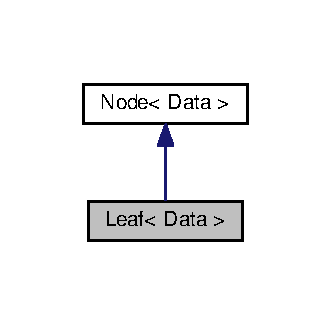
\includegraphics[width=159pt]{classLeaf__inherit__graph}
\end{center}
\end{figure}


Collaboration diagram for Leaf$<$ Data $>$\+:\nopagebreak
\begin{figure}[H]
\begin{center}
\leavevmode
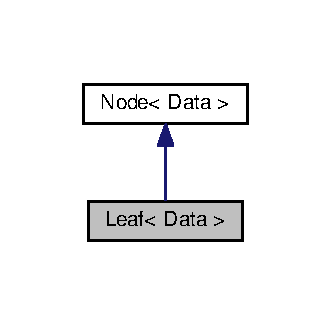
\includegraphics[width=159pt]{classLeaf__coll__graph}
\end{center}
\end{figure}
\subsection*{Public Member Functions}
\begin{DoxyCompactItemize}
\item 
\hyperlink{classLeaf_a455e433aabda9fc86ca01592188fade6}{Leaf} ()
\begin{DoxyCompactList}\small\item\em Constructor por defecto. \end{DoxyCompactList}\item 
\hyperlink{classLeaf_a58d1028691698747e42b279374825eca}{Leaf} (int \hyperlink{classNode_a672764de1b85ccfcb1c55429b5efbb1a}{order})
\begin{DoxyCompactList}\small\item\em Constructor para crear una Hoja de un tamanno pre establecido. \end{DoxyCompactList}\item 
\hyperlink{classLeaf_aa994510211d046a3b722c00c96e134a7}{Leaf} (int \hyperlink{classNode_a672764de1b85ccfcb1c55429b5efbb1a}{order}, \hyperlink{classNode}{Node}$<$ \hyperlink{main_8cpp_a0c209e815d35b218025a240523b4335b}{Data} $>$ $\ast$\hyperlink{classNode_ab8b577c94add9ebf4392c82301bcc49e}{father})
\begin{DoxyCompactList}\small\item\em Constructor por copia. \end{DoxyCompactList}\item 
virtual \hyperlink{classLeaf_a8ed11130cae158ab5eae6d2ed5502e52}{$\sim$\+Leaf} ()
\begin{DoxyCompactList}\small\item\em Destructor. \end{DoxyCompactList}\end{DoxyCompactItemize}
\subsection*{Data Fields}
\begin{DoxyCompactItemize}
\item 
\hyperlink{main_8cpp_a0c209e815d35b218025a240523b4335b}{Data} $\ast$ \hyperlink{classLeaf_a2ab8ad24d9d54d66b62e4ec4f89e32dc}{array\+Data}
\end{DoxyCompactItemize}


\subsection{Constructor \& Destructor Documentation}
\index{Leaf@{Leaf}!Leaf@{Leaf}}
\index{Leaf@{Leaf}!Leaf@{Leaf}}
\subsubsection[{\texorpdfstring{Leaf()}{Leaf()}}]{\setlength{\rightskip}{0pt plus 5cm}template$<$typename Data$>$ {\bf Leaf}$<$ {\bf Data} $>$\+::{\bf Leaf} (
\begin{DoxyParamCaption}
{}
\end{DoxyParamCaption}
)\hspace{0.3cm}{\ttfamily [inline]}}\hypertarget{classLeaf_a455e433aabda9fc86ca01592188fade6}{}\label{classLeaf_a455e433aabda9fc86ca01592188fade6}


Constructor por defecto. 

\index{Leaf@{Leaf}!Leaf@{Leaf}}
\index{Leaf@{Leaf}!Leaf@{Leaf}}
\subsubsection[{\texorpdfstring{Leaf(int order)}{Leaf(int order)}}]{\setlength{\rightskip}{0pt plus 5cm}template$<$typename Data$>$ {\bf Leaf}$<$ {\bf Data} $>$\+::{\bf Leaf} (
\begin{DoxyParamCaption}
\item[{int}]{order}
\end{DoxyParamCaption}
)\hspace{0.3cm}{\ttfamily [inline]}}\hypertarget{classLeaf_a58d1028691698747e42b279374825eca}{}\label{classLeaf_a58d1028691698747e42b279374825eca}


Constructor para crear una Hoja de un tamanno pre establecido. 

\index{Leaf@{Leaf}!Leaf@{Leaf}}
\index{Leaf@{Leaf}!Leaf@{Leaf}}
\subsubsection[{\texorpdfstring{Leaf(int order, Node$<$ Data $>$ $\ast$father)}{Leaf(int order, Node< Data > *father)}}]{\setlength{\rightskip}{0pt plus 5cm}template$<$typename Data$>$ {\bf Leaf}$<$ {\bf Data} $>$\+::{\bf Leaf} (
\begin{DoxyParamCaption}
\item[{int}]{order, }
\item[{{\bf Node}$<$ {\bf Data} $>$ $\ast$}]{father}
\end{DoxyParamCaption}
)\hspace{0.3cm}{\ttfamily [inline]}}\hypertarget{classLeaf_aa994510211d046a3b722c00c96e134a7}{}\label{classLeaf_aa994510211d046a3b722c00c96e134a7}


Constructor por copia. 

\index{Leaf@{Leaf}!````~Leaf@{$\sim$\+Leaf}}
\index{````~Leaf@{$\sim$\+Leaf}!Leaf@{Leaf}}
\subsubsection[{\texorpdfstring{$\sim$\+Leaf()}{~Leaf()}}]{\setlength{\rightskip}{0pt plus 5cm}template$<$typename Data$>$ virtual {\bf Leaf}$<$ {\bf Data} $>$\+::$\sim${\bf Leaf} (
\begin{DoxyParamCaption}
{}
\end{DoxyParamCaption}
)\hspace{0.3cm}{\ttfamily [inline]}, {\ttfamily [virtual]}}\hypertarget{classLeaf_a8ed11130cae158ab5eae6d2ed5502e52}{}\label{classLeaf_a8ed11130cae158ab5eae6d2ed5502e52}


Destructor. 



\subsection{Field Documentation}
\index{Leaf@{Leaf}!array\+Data@{array\+Data}}
\index{array\+Data@{array\+Data}!Leaf@{Leaf}}
\subsubsection[{\texorpdfstring{array\+Data}{arrayData}}]{\setlength{\rightskip}{0pt plus 5cm}template$<$typename Data$>$ {\bf Data}$\ast$ {\bf Leaf}$<$ {\bf Data} $>$\+::array\+Data}\hypertarget{classLeaf_a2ab8ad24d9d54d66b62e4ec4f89e32dc}{}\label{classLeaf_a2ab8ad24d9d54d66b62e4ec4f89e32dc}


The documentation for this class was generated from the following file\+:\begin{DoxyCompactItemize}
\item 
\hyperlink{Leaf_8h}{Leaf.\+h}\end{DoxyCompactItemize}

\hypertarget{classNode}{}\section{Node$<$ Data $>$ Class Template Reference}
\label{classNode}\index{Node$<$ Data $>$@{Node$<$ Data $>$}}


{\ttfamily \#include $<$Node.\+h$>$}



Inheritance diagram for Node$<$ Data $>$\+:\nopagebreak
\begin{figure}[H]
\begin{center}
\leavevmode
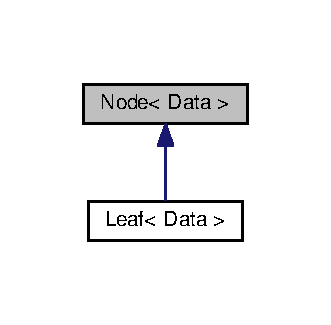
\includegraphics[width=159pt]{classNode__inherit__graph}
\end{center}
\end{figure}
\subsection*{Public Member Functions}
\begin{DoxyCompactItemize}
\item 
\hyperlink{classNode_a3e22ca89f75595b6020cfec6f05a8180}{Node} ()
\begin{DoxyCompactList}\small\item\em Constructor por defecto. \end{DoxyCompactList}\item 
\hyperlink{classNode_a69d52c1e2617398842a8fe1b009a16dd}{Node} (int \hyperlink{classNode_a672764de1b85ccfcb1c55429b5efbb1a}{order})
\begin{DoxyCompactList}\small\item\em Constructor para crear un Nodo de un tamanno pre establecido. \end{DoxyCompactList}\item 
\hyperlink{classNode_a0392b47c786821da7820c3a335cf9a21}{Node} (int \hyperlink{classNode_a672764de1b85ccfcb1c55429b5efbb1a}{order}, \hyperlink{classNode}{Node}$<$ \hyperlink{main_8cpp_a0c209e815d35b218025a240523b4335b}{Data} $>$ $\ast$\hyperlink{classNode_ab8b577c94add9ebf4392c82301bcc49e}{father})
\begin{DoxyCompactList}\small\item\em Constructor por copia. \end{DoxyCompactList}\item 
virtual \hyperlink{classNode_a726c47a8f963f9dc9e5d4b3ed3a63226}{$\sim$\+Node} ()
\begin{DoxyCompactList}\small\item\em Destructor. \end{DoxyCompactList}\end{DoxyCompactItemize}
\subsection*{Data Fields}
\begin{DoxyCompactItemize}
\item 
int \hyperlink{classNode_a78a7edbe6baf7950b4b937baf3a8977c}{elements}
\item 
int \hyperlink{classNode_a672764de1b85ccfcb1c55429b5efbb1a}{order}
\item 
int \hyperlink{classNode_add792264f859e503c01ad702e579c5b2}{is\+Leaf}
\item 
int $\ast$ \hyperlink{classNode_a89c4e4985e29c218d98bcb2dca481476}{array\+Keys}
\item 
\hyperlink{classNode}{Node}$<$ \hyperlink{main_8cpp_a0c209e815d35b218025a240523b4335b}{Data} $>$ $\ast$$\ast$ \hyperlink{classNode_a9dfc15b1a1835593b1061ba5d6685a20}{array\+Ptrs}
\item 
\hyperlink{classNode}{Node}$<$ \hyperlink{main_8cpp_a0c209e815d35b218025a240523b4335b}{Data} $>$ $\ast$ \hyperlink{classNode_ab8b577c94add9ebf4392c82301bcc49e}{father}
\end{DoxyCompactItemize}


\subsection{Constructor \& Destructor Documentation}
\index{Node@{Node}!Node@{Node}}
\index{Node@{Node}!Node@{Node}}
\subsubsection[{\texorpdfstring{Node()}{Node()}}]{\setlength{\rightskip}{0pt plus 5cm}template$<$typename Data$>$ {\bf Node}$<$ {\bf Data} $>$\+::{\bf Node} (
\begin{DoxyParamCaption}
{}
\end{DoxyParamCaption}
)\hspace{0.3cm}{\ttfamily [inline]}}\hypertarget{classNode_a3e22ca89f75595b6020cfec6f05a8180}{}\label{classNode_a3e22ca89f75595b6020cfec6f05a8180}


Constructor por defecto. 

\index{Node@{Node}!Node@{Node}}
\index{Node@{Node}!Node@{Node}}
\subsubsection[{\texorpdfstring{Node(int order)}{Node(int order)}}]{\setlength{\rightskip}{0pt plus 5cm}template$<$typename Data$>$ {\bf Node}$<$ {\bf Data} $>$\+::{\bf Node} (
\begin{DoxyParamCaption}
\item[{int}]{order}
\end{DoxyParamCaption}
)\hspace{0.3cm}{\ttfamily [inline]}}\hypertarget{classNode_a69d52c1e2617398842a8fe1b009a16dd}{}\label{classNode_a69d52c1e2617398842a8fe1b009a16dd}


Constructor para crear un Nodo de un tamanno pre establecido. 

\index{Node@{Node}!Node@{Node}}
\index{Node@{Node}!Node@{Node}}
\subsubsection[{\texorpdfstring{Node(int order, Node$<$ Data $>$ $\ast$father)}{Node(int order, Node< Data > *father)}}]{\setlength{\rightskip}{0pt plus 5cm}template$<$typename Data$>$ {\bf Node}$<$ {\bf Data} $>$\+::{\bf Node} (
\begin{DoxyParamCaption}
\item[{int}]{order, }
\item[{{\bf Node}$<$ {\bf Data} $>$ $\ast$}]{father}
\end{DoxyParamCaption}
)\hspace{0.3cm}{\ttfamily [inline]}}\hypertarget{classNode_a0392b47c786821da7820c3a335cf9a21}{}\label{classNode_a0392b47c786821da7820c3a335cf9a21}


Constructor por copia. 

\index{Node@{Node}!````~Node@{$\sim$\+Node}}
\index{````~Node@{$\sim$\+Node}!Node@{Node}}
\subsubsection[{\texorpdfstring{$\sim$\+Node()}{~Node()}}]{\setlength{\rightskip}{0pt plus 5cm}template$<$typename Data$>$ virtual {\bf Node}$<$ {\bf Data} $>$\+::$\sim${\bf Node} (
\begin{DoxyParamCaption}
{}
\end{DoxyParamCaption}
)\hspace{0.3cm}{\ttfamily [inline]}, {\ttfamily [virtual]}}\hypertarget{classNode_a726c47a8f963f9dc9e5d4b3ed3a63226}{}\label{classNode_a726c47a8f963f9dc9e5d4b3ed3a63226}


Destructor. 



\subsection{Field Documentation}
\index{Node@{Node}!array\+Keys@{array\+Keys}}
\index{array\+Keys@{array\+Keys}!Node@{Node}}
\subsubsection[{\texorpdfstring{array\+Keys}{arrayKeys}}]{\setlength{\rightskip}{0pt plus 5cm}template$<$typename Data$>$ int$\ast$ {\bf Node}$<$ {\bf Data} $>$\+::array\+Keys}\hypertarget{classNode_a89c4e4985e29c218d98bcb2dca481476}{}\label{classNode_a89c4e4985e29c218d98bcb2dca481476}
\index{Node@{Node}!array\+Ptrs@{array\+Ptrs}}
\index{array\+Ptrs@{array\+Ptrs}!Node@{Node}}
\subsubsection[{\texorpdfstring{array\+Ptrs}{arrayPtrs}}]{\setlength{\rightskip}{0pt plus 5cm}template$<$typename Data$>$ {\bf Node}$<${\bf Data}$>$$\ast$$\ast$ {\bf Node}$<$ {\bf Data} $>$\+::array\+Ptrs}\hypertarget{classNode_a9dfc15b1a1835593b1061ba5d6685a20}{}\label{classNode_a9dfc15b1a1835593b1061ba5d6685a20}
\index{Node@{Node}!elements@{elements}}
\index{elements@{elements}!Node@{Node}}
\subsubsection[{\texorpdfstring{elements}{elements}}]{\setlength{\rightskip}{0pt plus 5cm}template$<$typename Data$>$ int {\bf Node}$<$ {\bf Data} $>$\+::elements}\hypertarget{classNode_a78a7edbe6baf7950b4b937baf3a8977c}{}\label{classNode_a78a7edbe6baf7950b4b937baf3a8977c}
\index{Node@{Node}!father@{father}}
\index{father@{father}!Node@{Node}}
\subsubsection[{\texorpdfstring{father}{father}}]{\setlength{\rightskip}{0pt plus 5cm}template$<$typename Data$>$ {\bf Node}$<${\bf Data}$>$$\ast$ {\bf Node}$<$ {\bf Data} $>$\+::father}\hypertarget{classNode_ab8b577c94add9ebf4392c82301bcc49e}{}\label{classNode_ab8b577c94add9ebf4392c82301bcc49e}
\index{Node@{Node}!is\+Leaf@{is\+Leaf}}
\index{is\+Leaf@{is\+Leaf}!Node@{Node}}
\subsubsection[{\texorpdfstring{is\+Leaf}{isLeaf}}]{\setlength{\rightskip}{0pt plus 5cm}template$<$typename Data$>$ int {\bf Node}$<$ {\bf Data} $>$\+::is\+Leaf}\hypertarget{classNode_add792264f859e503c01ad702e579c5b2}{}\label{classNode_add792264f859e503c01ad702e579c5b2}
\index{Node@{Node}!order@{order}}
\index{order@{order}!Node@{Node}}
\subsubsection[{\texorpdfstring{order}{order}}]{\setlength{\rightskip}{0pt plus 5cm}template$<$typename Data$>$ int {\bf Node}$<$ {\bf Data} $>$\+::order}\hypertarget{classNode_a672764de1b85ccfcb1c55429b5efbb1a}{}\label{classNode_a672764de1b85ccfcb1c55429b5efbb1a}


The documentation for this class was generated from the following file\+:\begin{DoxyCompactItemize}
\item 
\hyperlink{Node_8h}{Node.\+h}\end{DoxyCompactItemize}

\chapter{File Documentation}
\hypertarget{BPlusTree_8h}{}\section{B\+Plus\+Tree.\+h File Reference}
\label{BPlusTree_8h}\index{B\+Plus\+Tree.\+h@{B\+Plus\+Tree.\+h}}
{\ttfamily \#include $<$cmath$>$}\\*
{\ttfamily \#include $<$iostream$>$}\\*
{\ttfamily \#include \char`\"{}Node.\+h\char`\"{}}\\*
{\ttfamily \#include \char`\"{}Leaf.\+h\char`\"{}}\\*
Include dependency graph for B\+Plus\+Tree.\+h\+:\nopagebreak
\begin{figure}[H]
\begin{center}
\leavevmode
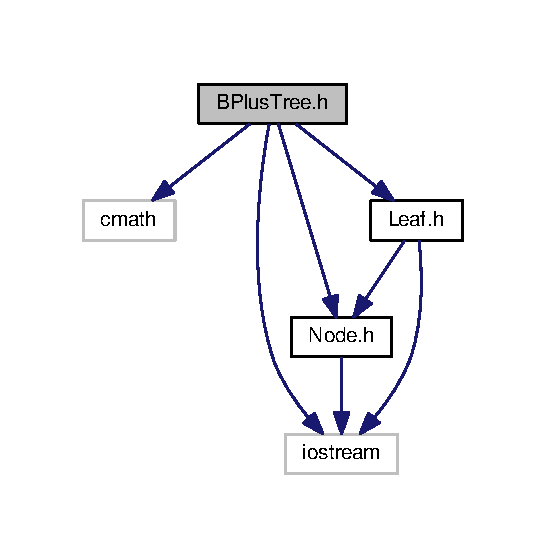
\includegraphics[width=262pt]{BPlusTree_8h__incl}
\end{center}
\end{figure}
This graph shows which files directly or indirectly include this file\+:\nopagebreak
\begin{figure}[H]
\begin{center}
\leavevmode
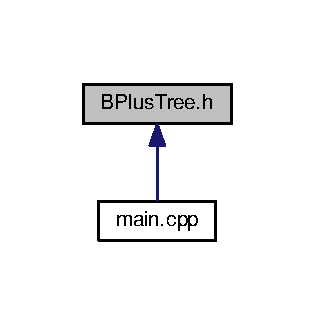
\includegraphics[width=151pt]{BPlusTree_8h__dep__incl}
\end{center}
\end{figure}
\subsection*{Data Structures}
\begin{DoxyCompactItemize}
\item 
class \hyperlink{classBPlusTree}{B\+Plus\+Tree$<$ Data $>$}
\end{DoxyCompactItemize}

\hypertarget{Leaf_8h}{}\section{Leaf.\+h File Reference}
\label{Leaf_8h}\index{Leaf.\+h@{Leaf.\+h}}
{\ttfamily \#include $<$iostream$>$}\\*
{\ttfamily \#include \char`\"{}Node.\+h\char`\"{}}\\*
Include dependency graph for Leaf.\+h\+:\nopagebreak
\begin{figure}[H]
\begin{center}
\leavevmode
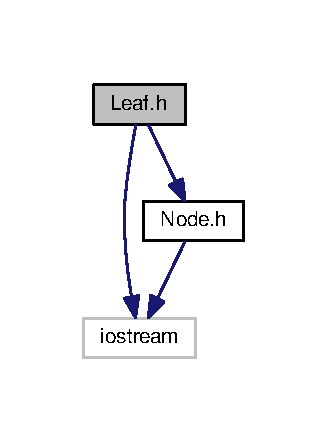
\includegraphics[width=157pt]{Leaf_8h__incl}
\end{center}
\end{figure}
This graph shows which files directly or indirectly include this file\+:\nopagebreak
\begin{figure}[H]
\begin{center}
\leavevmode
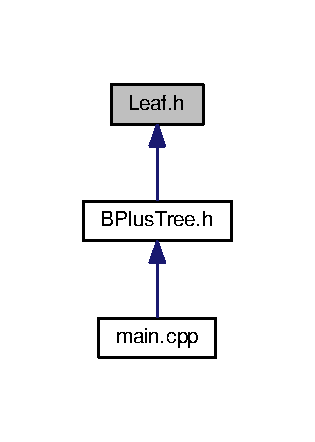
\includegraphics[width=151pt]{Leaf_8h__dep__incl}
\end{center}
\end{figure}
\subsection*{Data Structures}
\begin{DoxyCompactItemize}
\item 
class \hyperlink{classLeaf}{Leaf$<$ Data $>$}
\end{DoxyCompactItemize}

\hypertarget{main_8cpp}{}\section{main.\+cpp File Reference}
\label{main_8cpp}\index{main.\+cpp@{main.\+cpp}}
{\ttfamily \#include $<$stdlib.\+h$>$}\\*
{\ttfamily \#include \char`\"{}Controlador.\+h\char`\"{}}\\*
Include dependency graph for main.\+cpp\+:\nopagebreak
\begin{figure}[H]
\begin{center}
\leavevmode
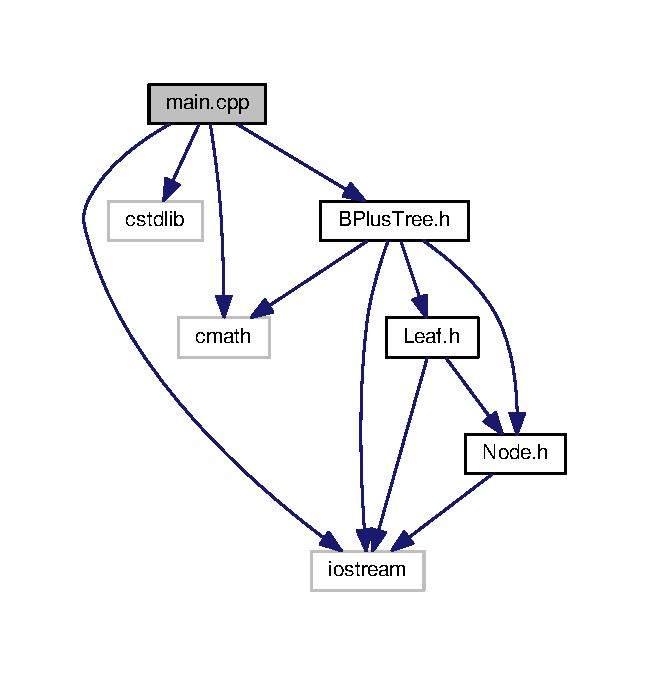
\includegraphics[width=350pt]{main_8cpp__incl}
\end{center}
\end{figure}
\subsection*{Functions}
\begin{DoxyCompactItemize}
\item 
int \hyperlink{main_8cpp_a0ddf1224851353fc92bfbff6f499fa97}{main} (int argc, char $\ast$argv\mbox{[}$\,$\mbox{]})
\end{DoxyCompactItemize}


\subsection{Function Documentation}
\index{main.\+cpp@{main.\+cpp}!main@{main}}
\index{main@{main}!main.\+cpp@{main.\+cpp}}
\subsubsection[{\texorpdfstring{main(int argc, char $\ast$argv[])}{main(int argc, char *argv[])}}]{\setlength{\rightskip}{0pt plus 5cm}int main (
\begin{DoxyParamCaption}
\item[{int}]{argc, }
\item[{char $\ast$}]{argv\mbox{[}$\,$\mbox{]}}
\end{DoxyParamCaption}
)}\hypertarget{main_8cpp_a0ddf1224851353fc92bfbff6f499fa97}{}\label{main_8cpp_a0ddf1224851353fc92bfbff6f499fa97}

\hypertarget{Node_8h}{}\section{Node.\+h File Reference}
\label{Node_8h}\index{Node.\+h@{Node.\+h}}


Clase Arbol\+B+.  


{\ttfamily \#include $<$iostream$>$}\\*
Include dependency graph for Node.\+h\+:\nopagebreak
\begin{figure}[H]
\begin{center}
\leavevmode
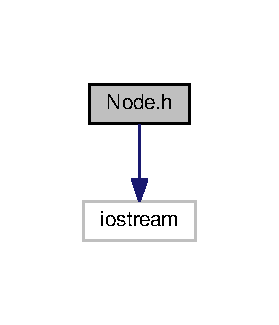
\includegraphics[width=134pt]{Node_8h__incl}
\end{center}
\end{figure}
This graph shows which files directly or indirectly include this file\+:
\nopagebreak
\begin{figure}[H]
\begin{center}
\leavevmode
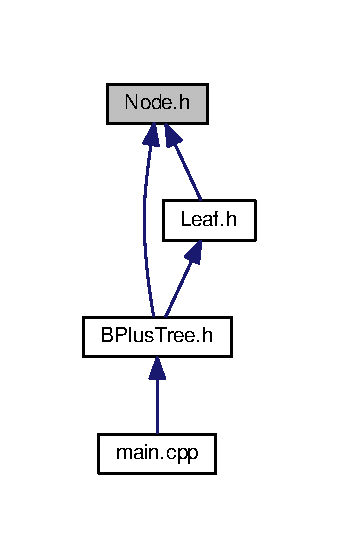
\includegraphics[width=163pt]{Node_8h__dep__incl}
\end{center}
\end{figure}
\subsection*{Data Structures}
\begin{DoxyCompactItemize}
\item 
class \hyperlink{classNode}{Node$<$ Data $>$}
\end{DoxyCompactItemize}


\subsection{Detailed Description}
Clase Arbol\+B+. 

Clase Nodo.

Clase main.

Clase Hoja.

\begin{DoxyVersion}{Version}
1.\+0 
\end{DoxyVersion}
\begin{DoxyDate}{Date}
6/03/17 
\end{DoxyDate}
\begin{DoxyAuthor}{Author}
Luis Diego Fernandez, Daniel Jimenez  Arbol B+ 
\end{DoxyAuthor}

%--- End generated contents ---

% Index
\backmatter
\newpage
\phantomsection
\clearemptydoublepage
\addcontentsline{toc}{chapter}{Index}
\printindex

\end{document}
